\subsubsection{Total number of messages sent}\label{subsubsec:hd2krmessages}

This is an indication of the energy efficiency of the entire network.

The maximum number of copies is the dominant factor (\(58\%\)), as expected.
Also the size of the hear window \(T\) and its combination with the maximum
number of copies have a valuable impact on this index. The unexplained variation
is less than \(1\%\).

In \figref{subfig:hdperfmessagesm} we see that the total number of messages sent
decreases with an lower value of the \code{maxCopies} parameter, as expected.
We note that with \(m\!=\!7\) we get that nearly all the users of the network
relay the message. In \figref{subfig:hdperfmessagesT} we can see that less
messages are sent if an higher size for the hear window is used when
\(m\!=\!3\). So, with a low \(m\), we can further decrease the total number of
messages sent by increasing \(T\). We expect \(T\) to hugely affect the total
broadcast time, so the selection of the factor \(T\) is a trade-off between the
energy efficiency and the total broadcast time.

\begin{figure}[htb]
	\centering
	\begin{subfigure}[b]{0.49\textwidth}
		\centering
		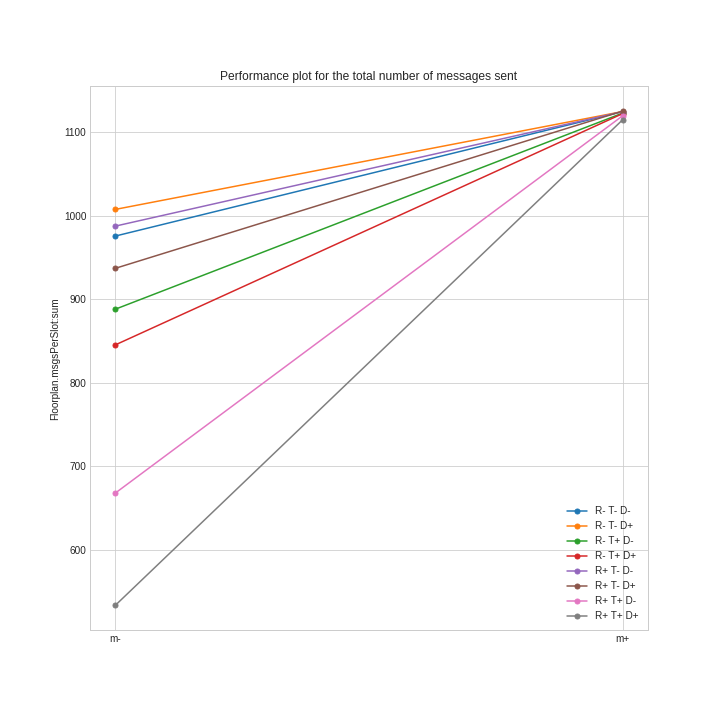
\includegraphics[width=\textwidth]{img/hd/messages-m-perfplot}
		\caption{When the maximum number of copies is reduced the total
		number of messages sent decreases}\label{subfig:hdperfmessagesm}
	\end{subfigure}
	\begin{subfigure}[b]{0.49\textwidth}
		\centering
		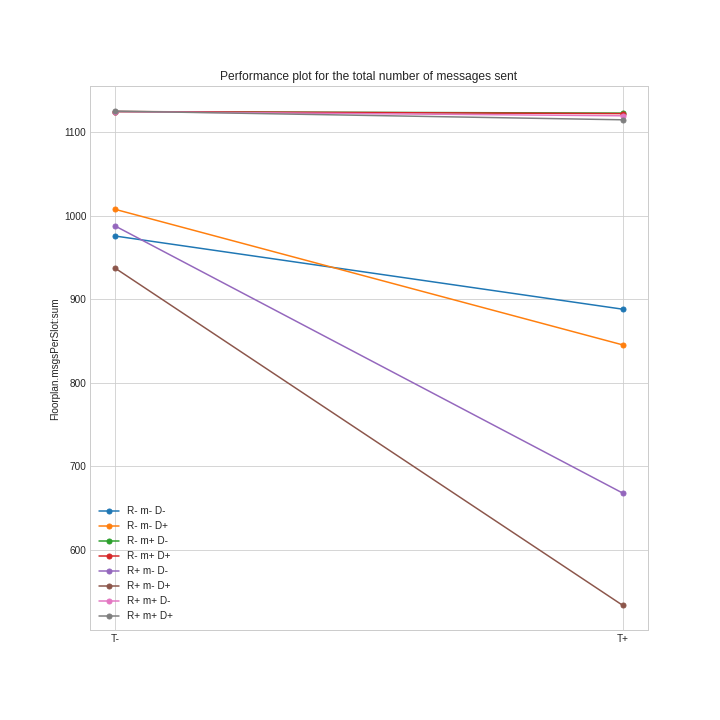
\includegraphics[width=\textwidth]{img/hd/messages-T-perfplot}
		\caption{Increase the size of the hear window to reduce the
		total number of messages sent}\label{subfig:hdperfmessagesT}
	\end{subfigure}
	\caption{Performance plots for the total number of messages
	sent}\label{fig:hdperfmessages}
\end{figure}
